\glsreset{cbf}
This chapter establishes the fundamentals for a system ensuring safety when a surgeon operates on a patient with a beating heart. In addition to the safety, it is the objective to found a system such that the surgeon experiences a beating heart as static. As indicated in \autoref{sec:aau_doc}, a proper initial set-up could be a surface mounted on a cylinder moving periodically as a sinusoid (in contrast to a more advanced (realistic) model of the heart, such as the one described in \autoref{app:dynamic_model_heart}). The scheme is outlined in \autoref{fig:dynamic_overview}.
\vspace{-2mm}
\begin{figure}[H]
%\hspace*{-10mm}
\subbottom[Terms]{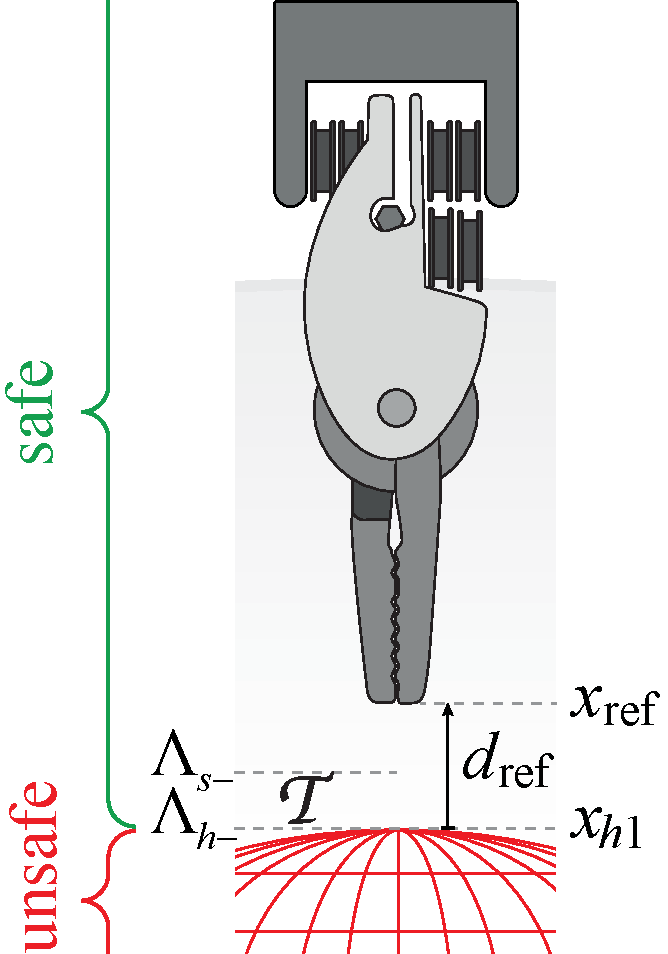
\includegraphics[height=4.2cm]{dynamic_boundary_limits.pdf}\label{fig:over_1}} \hspace{0.5cm}
\subbottom[Time sequence of a tool following a relative reference $d_\text{ref}$]{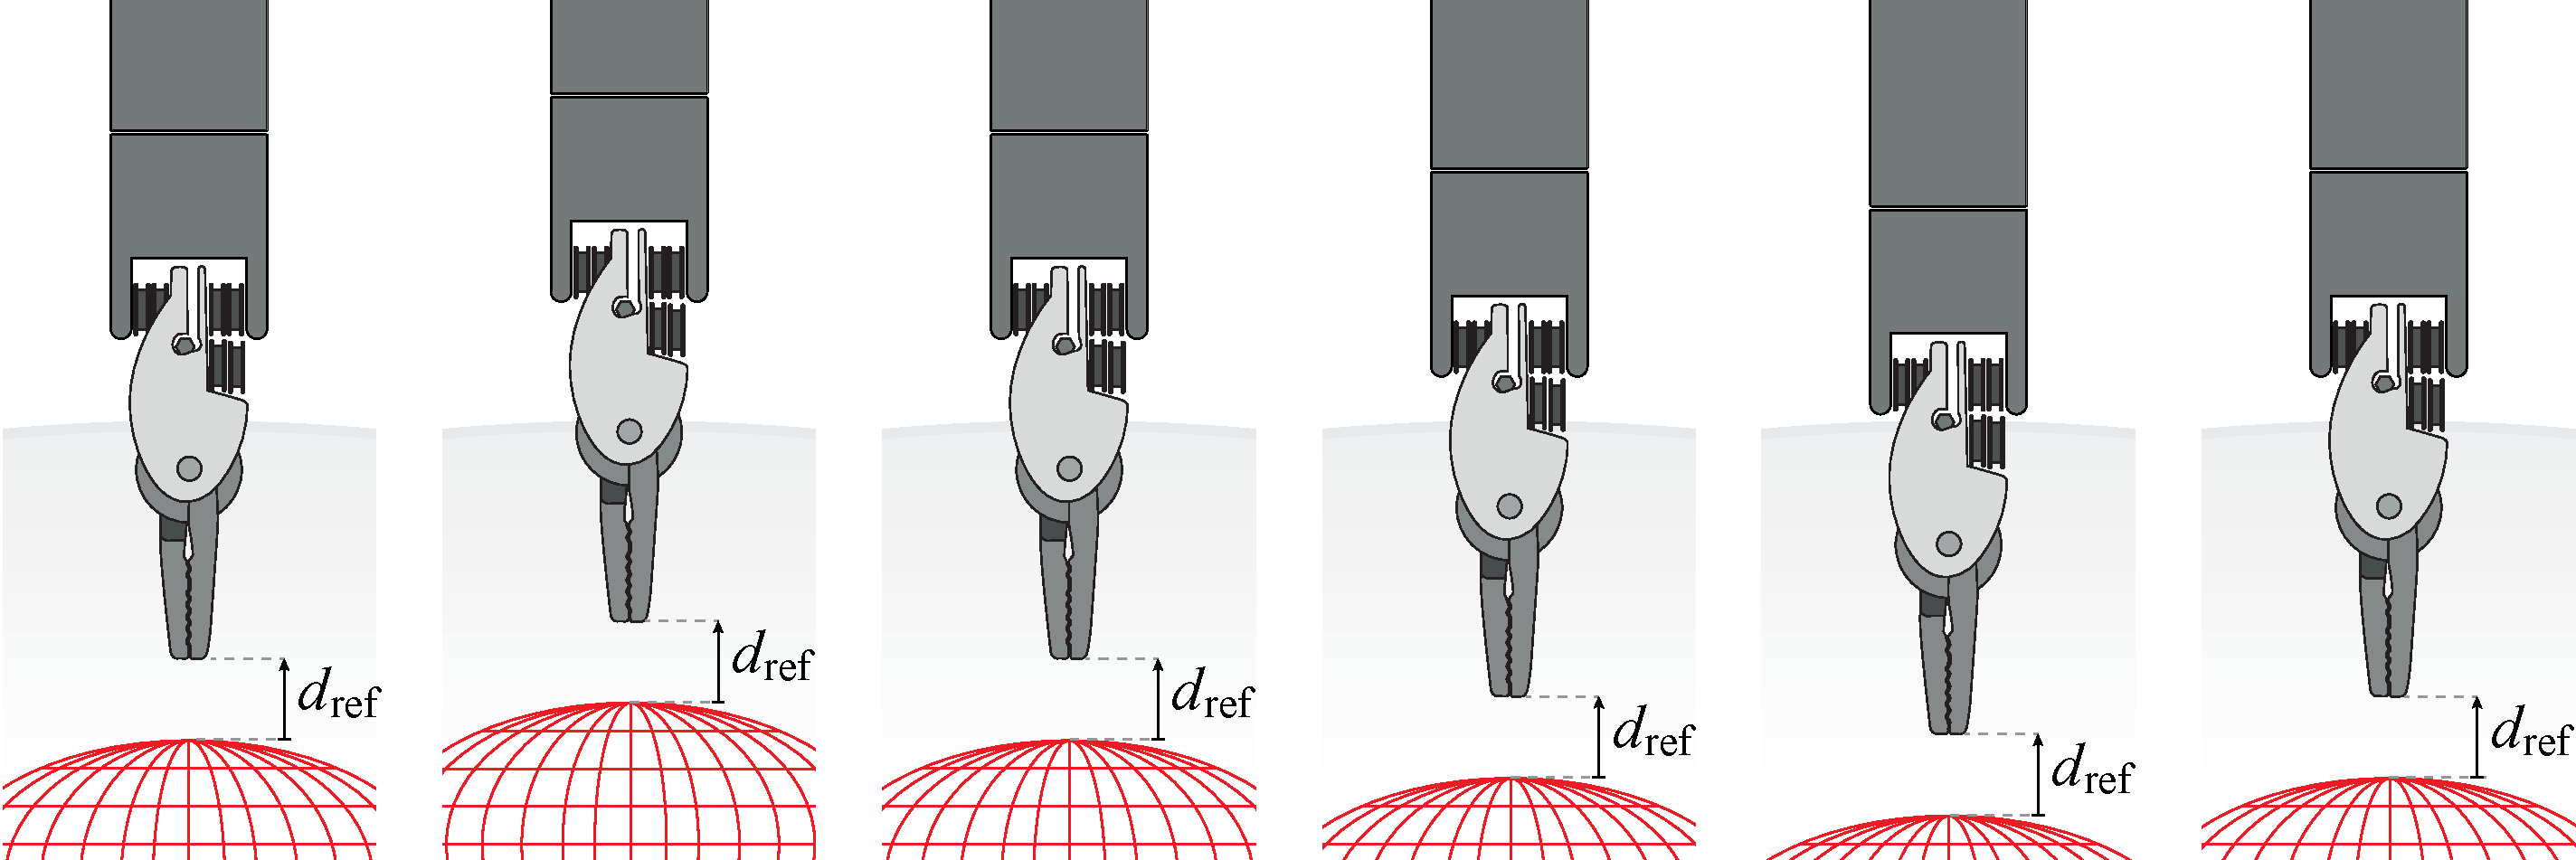
\includegraphics[height=4.2cm]{dynamic_boundary_sequence.pdf}\label{fig:over_2}}%
\caption{The objective is to control the distance to the object by following a relative reference $d_\text{ref}$, such that the surgeon experiences the object as static and can operate as if the object was in fact standing still. An overview of terms applied is found in \autoref{fig:over_1}.}
\label{fig:dynamic_overview}
\end{figure}
Thus a model of a beating heart will first be outlined.
%\begin{figure}[H]
%	\center
%		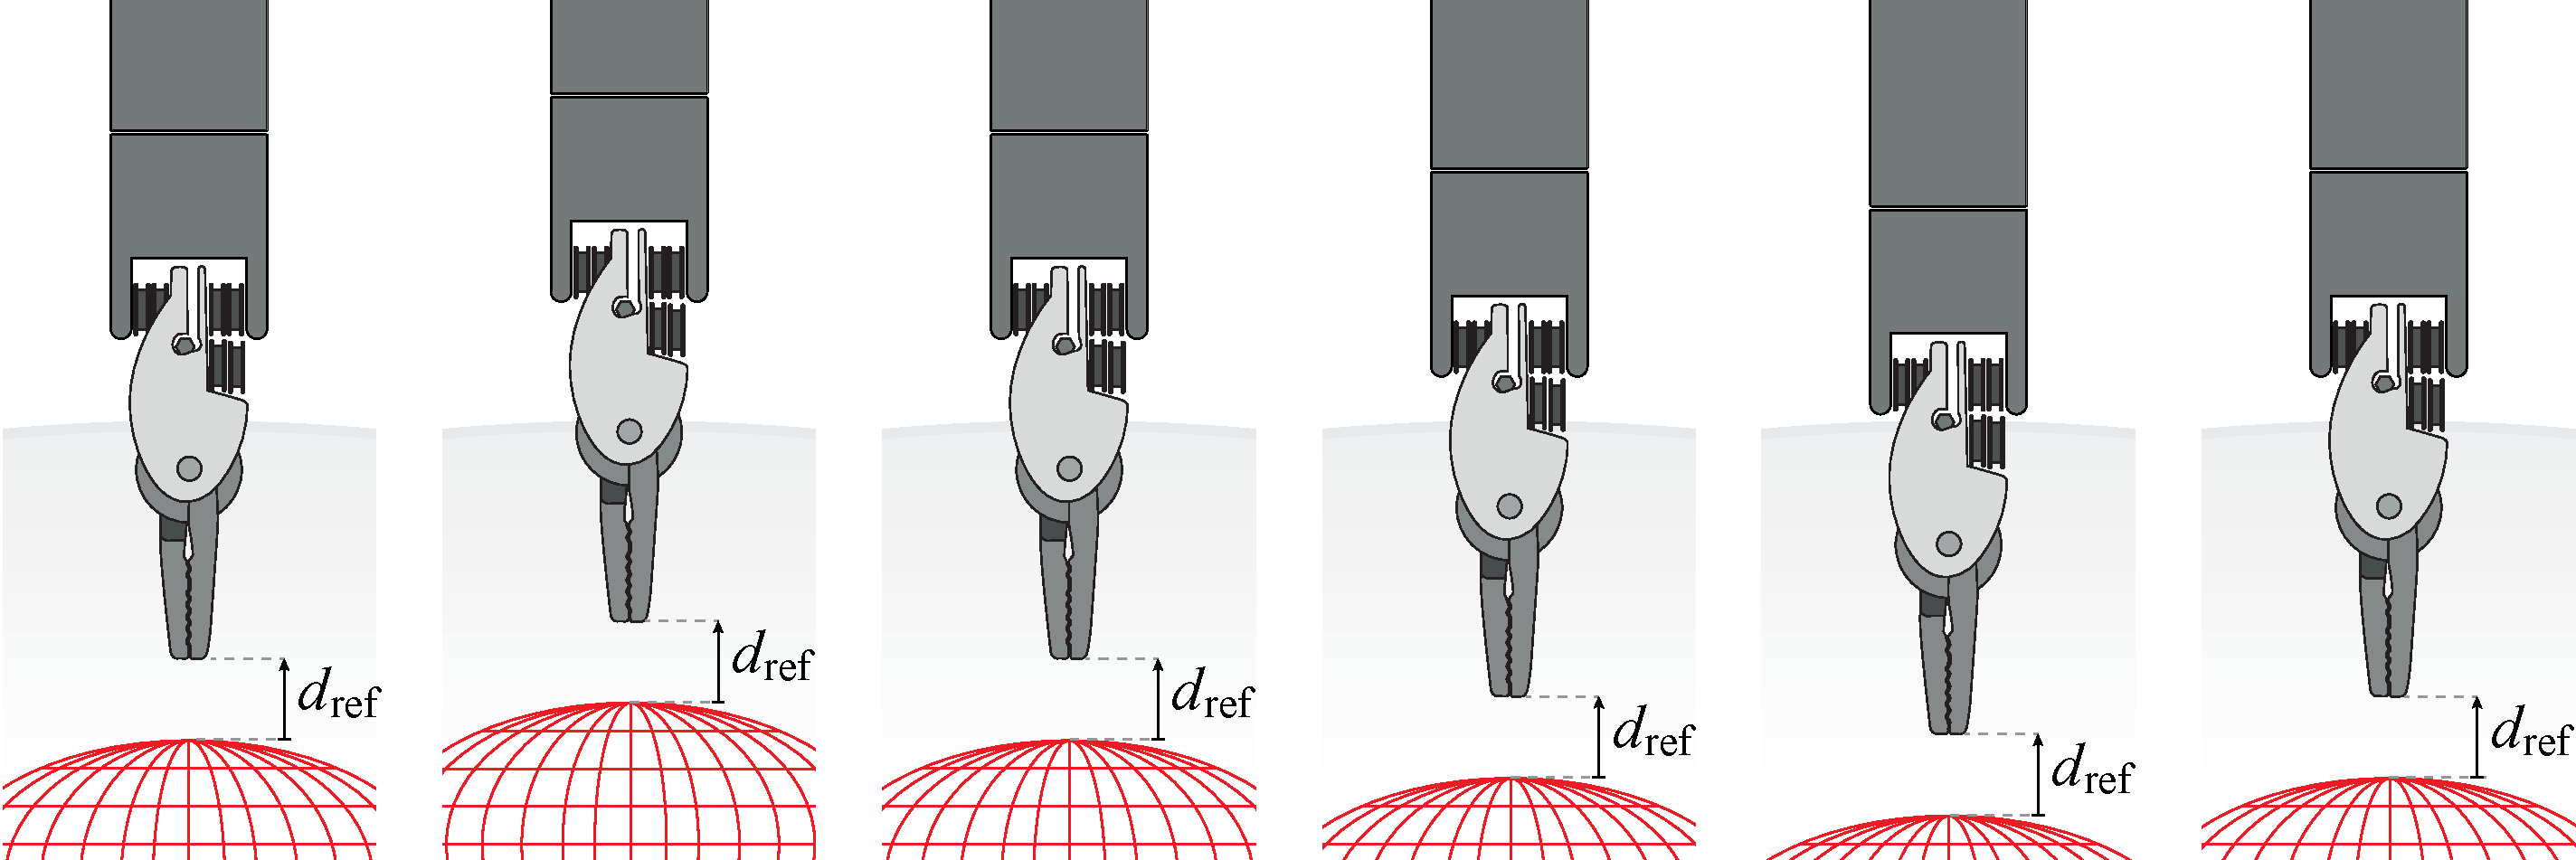
\includegraphics[width=1\textwidth]{dynamic_boundary_sequence.pdf}
%	\caption{lol.}
%	\label{fig:dynamic_overview}
%\end{figure}
%and..
%\begin{figure}[H]
%	\center
%		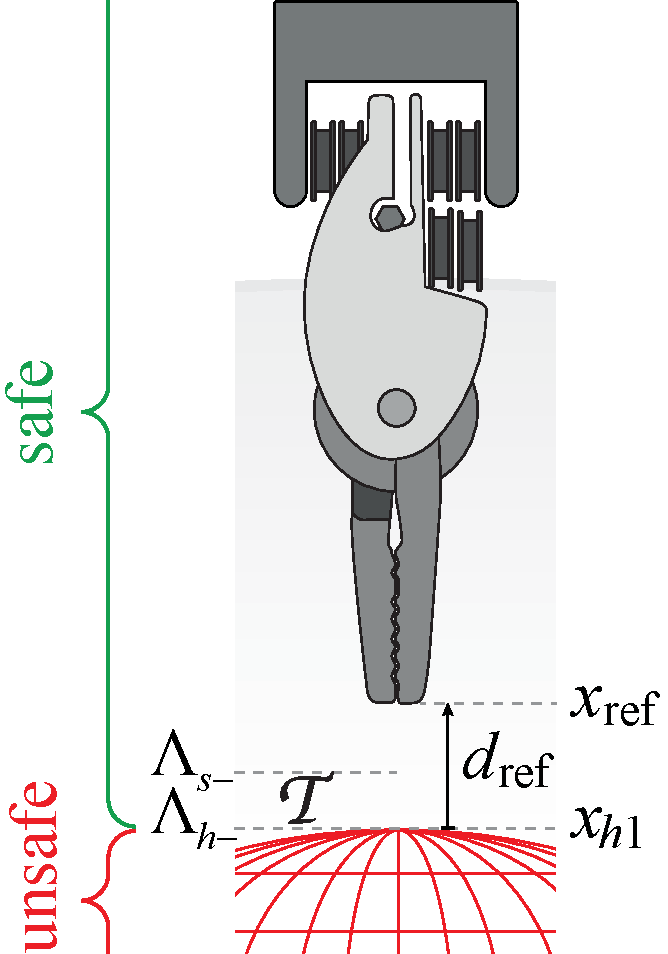
\includegraphics[width=0.2\textwidth]{dynamic_boundary_limits.pdf}
%	\caption{lol.}
%	\label{fig:dynamic_overview_2}
%\end{figure}
\subsubsection*{Modelling the Beating Heart}
\vspace{-2mm}
The simplified heart movement can be represented as a matrix with eigenvalues on the imaginary axis in the complex frequency domain:
\begin{flalign}
\dot{\textbf{x}}_h =
\dot{\begin{bmatrix}
x_{h1}\\x_{h2}
\end{bmatrix}} =
\begin{bmatrix}
0 & \omega_h \\ -\omega_h & 0
\end{bmatrix}
\begin{bmatrix}
x_{h1}\\x_{h2}
\end{bmatrix} \kk \text{with} \kk \mathbf{x}_{h}(0) =\begin{bmatrix}
x_{h10} \\
x_{h20}
\end{bmatrix}
\label{eq:beating_heart_sine}
\end{flalign}
\begin{tabular}{rp{14cm}} 
where  &  \\
$x_{h1}$& is the position of a point on the surface of the heart \\
$x_{h2}$& is the velocity of the point \\
$\omega_h$& is the heartbeat frequency, $\omega_h = 2\pi/T_h$ rad/s with an average heartbeat period $T_h=1.1$\,s \citep{bib:heart_berkeley} \\
$x_{h10}$ & is the initial value of $x_{h1}$ \\
$x_{h20}$ & is the initial value of $x_{h2}$\\
\end{tabular}\\


Note that the magnitude of $\omega_h$ determines the frequency and that the initial conditions determines the amplitude of the heart oscillation. The heartbeat will with this system have a natural oscillation around zero. 
\subsubsection*{Modelling the Robot Slide Movement}
\vspace{-1mm}
To model the one dimensional robot movement along the slide axis, the same system model can be used as presented in \autoref{eq:1storder_1D_ss}, i.e.:
\vspace{-3mm}
\begin{flalign}
\dot{x_1} = -\tau^{-1} x_1 + \tau^{-1} u
\label{eq:good_old}
\end{flalign}

\vspace{-1mm}
The one dimensional model is used to simplify the equations thus precluding complications at this stage. Additionally, the second order model merely proved few advantages in the form of elimination of the overshoot.
\vspace{-1mm}
\subsubsection*{Introducing a Dynamic Reference in the Model}
\vspace{-1mm}
To be able to guarantee that a given distance is maintained between the heart and the robot end effector, an additional state can be added the system. Thus, a new set of states is introduced representing the movement of the beating heart, the movement of the robot and a relative distance $d_\text{ref}$.
%\begin{flalign*}
%\textbf{x} = \begin{bmatrix}
%x_1 \\ x_{h1} \\ x_{h2} \\ d_\text{ref}
%\end{bmatrix}
%\end{flalign*}
Combining \autoref{eq:beating_heart_sine} and \autoref{eq:good_old} with the relative distance yields the below stated linear state space system: 
\vspace{-3mm}
\begin{flalign}
\dot{\textbf{x}}(t) &= \dot{\begin{bmatrix}
	x_1\\x_{h1}\\x_{h2}\\ d_\text{ref}
	\end{bmatrix}} =
\underbrace{\underbrace{\begin{bmatrix}
		-1/\tau & 0 & 0 & 0\\0 & 0 & \omega_h & 0 \\ 0 & -\omega_h & 0 & 0 \\ 0& 0 & 0 & 0
		\end{bmatrix}}_{\textbf{A}}
	\begin{bmatrix}
	x_1\\x_{h1}\\x_{h2}\\ d_\text{ref}
	\end{bmatrix}}_{f(\mathbf{x})}+ 
\underbrace{\underbrace{\begin{bmatrix}
		1/\tau \\ 0 \\ 0 \\ 0
		\end{bmatrix}}_{\textbf{B}}}_{g(\mathbf{x})} \tilde{u}(x) \\
		\mathbf{y}(t) &= \underbrace{\begin{bmatrix}
		1 & 0 & 0 & 0
		\end{bmatrix}}_\textbf{C} \textbf{x}(t)
\end{flalign}	
where the control law is introduced with the relative difference between robot position and heart position, i.e. $x_\text{ref} = x_{h1} + d_\text{ref}$ such that:
\vspace{-3mm}
\begin{flalign}
\tilde{u}(\mathbf{x}(t)) &= \bar{\mathbf{N}}x_\text{ref} - \mathbf{K}\,x_1 \nonumber\\
&= \bar{\mathbf{N}}\Big( x_{h1}(t)+ d_\text{ref} \Big)-\mathbf{K} x_1(t) \nonumber \\
%&= -\mathbf{K} x_1(t) + \bar{\mathbf{N}}x_{h1}(t) + \bar{\mathbf{N}} d_\text{ref}\nonumber \\
&= %\underbrace{
	\begin{bmatrix}
-\mathbf{K} & \bar{\mathbf{N}} & 0 & \bar{\mathbf{N}} 
\end{bmatrix}
%}_{\bar{\textbf{K}}} 
\textbf{x}(t) \nonumber\\
&= \bar{\textbf{K}} \textbf{x}(t)
\label{eq:utilde_dynamic}
\end{flalign}
\begin{tabular}{rl}
where &\\
$\tau$ & is the time constant of the first order system $\tau=0.11$\,s as given in \autoref{sec:model_slide}\\
$\mathbf{K}$ & is the linear system controller designed according to \autoref{eq:K_1}, $\mathbf{K} \in \mathbb{R}$ \\
$\bar{\textbf{N}}$ & is the system gain found according to \autoref{eq:barm_1}, $\bar{\mathbf{N}} \in \mathbb{R}$ \\
$\bar{\textbf{K}}$ & is the augmented feedback vector, $\bar{\textbf{K}} \in \mathbb{R}^{1 \times 4}$
\end{tabular}\\

%Such that:
%\begin{flalign}
%\tilde{u} = \bar{\textbf{K}} \textbf{x}
%\label{eq:utilde_dynamic}
%\end{flalign}
Note how the closed loop system can be rewritten in a more intuitive way, such that the system is reduced to three states taking $d_\text{ref}$ as input:
\vspace{-1mm}
\begin{flalign}
\dot{\begin{bmatrix}
	x_1\\x_{h1}\\x_{h2}\\d_\text{ref}
	\end{bmatrix}} &=
\underbrace{\underbrace{\begin{bmatrix}
		-1/\tau & 0 & 0 & 0\\0 & 0 & \omega_h & 0 \\ 0 & -\omega_h & 0 & 0 \\ 0& 0 & 0 & 0
		\end{bmatrix}}_{\textbf{A}}
	\begin{bmatrix}
	x_1\\x_{h1}\\x_{h2}\\d_\text{ref}
	\end{bmatrix}}_{f(\mathbf{x})}+ 
\underbrace{\underbrace{\begin{bmatrix}
		1/\tau \\ 0 \\ 0 \\ 0
		\end{bmatrix}}_{\textbf{B}}}_{g(\mathbf{x})}
\underbrace{\underbrace{\begin{bmatrix}
		-\mathbf{K} & \bar{\mathbf{N}} & 0 & \bar{\mathbf{N}}
		\end{bmatrix}}_{\bar{\textbf{K}}}
	\begin{bmatrix}
	x_1\\x_{h1}\\x_{h2}\\d_\text{ref}
	\end{bmatrix}}_{\tilde{u}(x)} \\
\dot{\begin{bmatrix}
	x_1\\x_{h1}\\x_{h2}
	\end{bmatrix}} &=
\underbrace{\begin{bmatrix}
	-(\mathbf{I}+\mathbf{K})/\tau & \bar{\mathbf{N}}/\tau & 0\\0 & 0 & \omega_h \\ 0 & -\omega_h & 0
	\end{bmatrix}}_{\textbf{A}_{cl}}
\begin{bmatrix}
x_1\\x_{h1}\\x_{h2}
\end{bmatrix}+ 
\underbrace{\begin{bmatrix}
	\bar{\mathbf{N}}/\tau \\ 0 \\ 0
	\end{bmatrix}}_{\textbf{B}_{cl}}
d_{ref}
\label{eq:cl_dynamic}
\end{flalign}
Note the eigenvalues of $\textbf{A}_{cl}$:
\vspace{-7mm}
\begin{flalign*}
\lambda_{\textbf{A}_{cl}} = \begin{cases}
-90 \\
5.71\,j \\
-5.71\,j
\end{cases}
\end{flalign*}
The eigenvalues reveal a stable (controllable) subsystem consisting of the robot end effector and an obviously marginally stable (uncontrollable) subsystem consisting of the beating heart.

This concludes the augmented system. Thus a \gls{cbf} will be constructed.
\vspace{-1mm}
\section{Construction of CBF}
\vspace{-3mm}
A barrier certificate for \autoref{eq:cl_dynamic} with a zero level set at the surface of the heart, comprises moving boundaries and hence should be a function of both robot and heart position. \Autoref{def:safety} implies that the \gls{cbf} should be constructed with unsafe region $\mathcal{X}_u$ below the surface of the heart, i.e. such that $B(x_1,x_{h1})$ is positive if $x_1<x_{h1}$ and negative otherwise. The coherence is clear:
\vspace{-1mm}
\begin{equation}
x_{h1} - x_1 > 0 \kk  \Rightarrow \kk \mathbf{x} \in \mathcal{X}_u \kk\Leftrightarrow\kk B(\mathbf{x}) > 0 \nonumber
%\\
%-x_1 + x_{h1} &> 0 \kk  \\
%x_{h1} - x_1 &> 0 
\end{equation}

\vspace{-2mm}
Thus a \gls{cbf} can be constructed as:
\vspace{-4mm}
\begin{flalign}
B(x_1,x_{h1})= \tilde{c}(x_{h1}-x_1)\label{eq:barrier_dynamic}
\end{flalign}

\vspace{-1mm}
with a positive constant $\tilde{c}>0$. Setting $\tilde{c} = 1$ yields a 1:1 mapping which indeed will be the case here. Thus according to \autoref{def:cbf} this is a valid CBF if $L_gB(\mathbf{x}) \neq 0$ and $\{\mathbf{x} \in \mathcal{X} | B( x_1 , x_{h1}) \leq 0 \} \neq \emptyset$. The latter  is trivial as the safe states are present if $d_\text{ref}>0$. Thus  $L_gB(x_1,x_{h1)}$ is analysed:
\begin{flalign}
L_gB(\mathbf{x}) = \frac{d B(x_1,x_{h1})}{ d \textbf{x}}g(\mathbf{x}) \Biggm|_{g(\mathbf{x}) = \textbf{B}}  
&= \begin{bmatrix}
\dfrac{\partial B(x_1,x_{h1})}{\partial x_1} & \dfrac{\partial B(x_1,x_{h1})}{\partial x_{h1}} & \dfrac{\partial B(x_1,x_{h1})}{\partial x_{h2}} & \dfrac{\partial B(x_1,x_{h1})}{\partial d_\text{ref}}
\end{bmatrix} \textbf{B} \nonumber \\
&= \begin{bmatrix}
-\tilde{c} & \tilde{c} & 0 & 0
\end{bmatrix}
\begin{bmatrix}
1/\tau\\
0 \\ 0 \\ 0
\end{bmatrix} \Bigm|_{\tilde{c}=1}  =
\frac{-1}{\tau} \neq 0 \quad \forall \, \mathbf{x} \in \mathcal{X}
\label{eq:lgb_dynamic}
\end{flalign}
It is seen that $L_gB(\mathbf{x}) \neq 0 \,\, \forall\,\, \mathbf{x} \in \mathcal{X}$. The \gls{cbf} is therefore valid on $\mathcal{X}$.
\section{Control Design}
The control law is, just as in \autoref{chap:cbf_1d_static}, split in two parts. A linear controller where no safety precautions are taken is used in $\mathcal{Y}$ and a controller ensuring safety is used in $\mathcal{T} \bigcup \mathcal{X}_u$. The controller ensuring safety is defined in \autoref{eq:control_law_safety}.

The transition between the two controllers in $\mathcal{T}$ is determined by $\sigma(\mathbf{x})$ which is defined in \autoref{eq:smoothness}. Thus a scalar $\epsilon$ is required. In this case, $\epsilon$ determines downright when the effect of the safety controller $k_0(\mathbf{x})$ is brought into effect, while the weighting of $k_0(\mathbf{x})$ is determined by $\sigma(\mathbf{x})$. To give the safety controller some margin to force the robot end effector away from $\mathcal{X}_u$, it is reasonable to let $k_0(\mathbf{x})$ take effect when the distance $d_\text{ref}$ reaches 1\,cm, thus:
\vspace{-3mm}
\begin{flalign}
\epsilon = 0.01\label{eq:epsilon_dynamic}
\end{flalign}

%\vspace{-3mm}
%Thus $\sigma(x)$ can be stated as:
%\begin{flalign}
%\sigma(x) = 
%\begin{cases}
%0 & \text{if} \mm B(x_1,x_{h1}) \leq -\epsilon \\
% -2  \left( \dfrac{B(x_1,x_{h1}}{\epsilon} \right)^3 - 3\left( \dfrac{B(x_1,x_{h1})}{\epsilon} \right)^2 +1  \kk &\text{if} \mm B(x_1,x_{h1}) \in (-\epsilon,0) \\
%1  &\text{if} \mm B(x_1,x_{h1}) \geq 0
%\end{cases}
%\label{eq:sig_dynamic}
%\end{flalign} 
The safety controller, as defined in \autoref{eq:control_law_safety}, requires  the Lie derivatives of the CBF, where $L_gB(\mathbf{x})$ is found in \autoref{eq:lgb_dynamic}, and $L_fB(\mathbf{x})$ is found as:
\begin{flalign}
L_fB(\mathbf{x}) &= \frac{dB(x_1,x_{h1})}{d\textbf{x}}f(\textbf{x})\Bigm|_{f(\textbf{x})=\textbf{A}\textbf{x}} \nonumber \\
&= \begin{bmatrix}
\dfrac{\partial  B(x_1,x_{h1})}{\partial x_1 } & \dfrac{\partial  B(x_1,x_{h1})}{\partial x_{1h} } & \dfrac{\partial  B(x_1,x_{h1})}{\partial x_{2h} } & \dfrac{\partial  B(x_1,x_{h1})}{\partial d_\text{ref} }
\end{bmatrix}  \begin{bmatrix}
1/\tau & 0 & 0 & 0 \\
0 & 0 & \omega_h & 0 \\
0 & -\omega_h & 0 & 0 \\
0 & 0 & 0 & 0 
\end{bmatrix} \begin{bmatrix}
x_1 \\ x_{x1} \\ x_{x2} \\ d_\text{ref}
\end{bmatrix} \nonumber \\
&=
\begin{bmatrix}
-\tilde{c} & \tilde{c} & 0 & 0
\end{bmatrix}
\begin{bmatrix}
-x_1/\tau\\
\omega_h x_{h2} \\
-\omega_h x_{h1} \\
0
\end{bmatrix} =
\tilde{c}\left(\omega_h x_{h2} + \frac{ x_1}{\tau}\right) \Bigm|_{\tilde{c}=1} = \omega_hx_{h2} + \dfrac{x_1}{\tau}
\label{eq:Lf_dynamic}
\end{flalign}

\begin{recap}[Control Law for Dynamic System with Relative Reference]
Using \autoref{eq:control_law}, the control law can be summarized as:
\begin{flalign*}
u(\mathbf{x}) = \sigma(\mathbf{x})k_0(\mathbf{x}) + (1-\sigma(\mathbf{x}))\tilde{u}(\mathbf{x})
\end{flalign*}
\begin{tabular}{rp{12.5cm}} 
where  &  \\
$\sigma(\mathbf{x})$ & is calculated from \autoref{eq:smoothness} with $B(\mathbf{x})$ found in \autoref{eq:barrier_dynamic} and $\epsilon$ found in \autoref{eq:epsilon_dynamic}\\
$k_0(\mathbf{x})$ & is calculated from \autoref{eq:control_law_safety} with the Lie derivatives from \ref{eq:lgb_dynamic} and \ref{eq:Lf_dynamic} \\
$\tilde{u}(\mathbf{x})$ & is calculated from \autoref{eq:utilde_dynamic}
\end{tabular}\\
\end{recap}
This completes the control design.

\section{MATLAB Results}
The results shown are implemented with the following characteristics:
\vspace{-2mm}
\begin{itemize}
	\itemsep-0.7mm
\item Extrapolation by means of forward Euler.
\item A sampling rate $f_s=2\,$kHz.
\item Simulation time for 5\,s.
\item The distance $d_\text{ref}$ is initially set to 3\,cm which is safe. At 2\,s the distance $d_\text{ref}$ is altered to -1\,cm emulating a surgeon who accidentally forced the robot to penetrate the heart. The expected outcome of this is obviously that the safety controller prevents this by ensuring a distance between end effector and the beating heart.
\item Initial conditions are set such that the robot end effector is positioned at a distance to the heart greater than the desired distance. The expected outcome is that the system will attempt to track the distance $x_1-x_{h1}=d_\text{ref}$.
\end{itemize}
The MATLAB implementation itself can be found in \autoref{app:slide_implement_1} and in \autoref{app:cd} under the path \texttt{matlab\_scripts/beating\_hearth/beating\_hearth\_controller.m}. The state trajectory is plotted in \autoref{fig:matlab_dynamics}.

\vspace{-2mm}
\begin{figure}[H]
	\center
		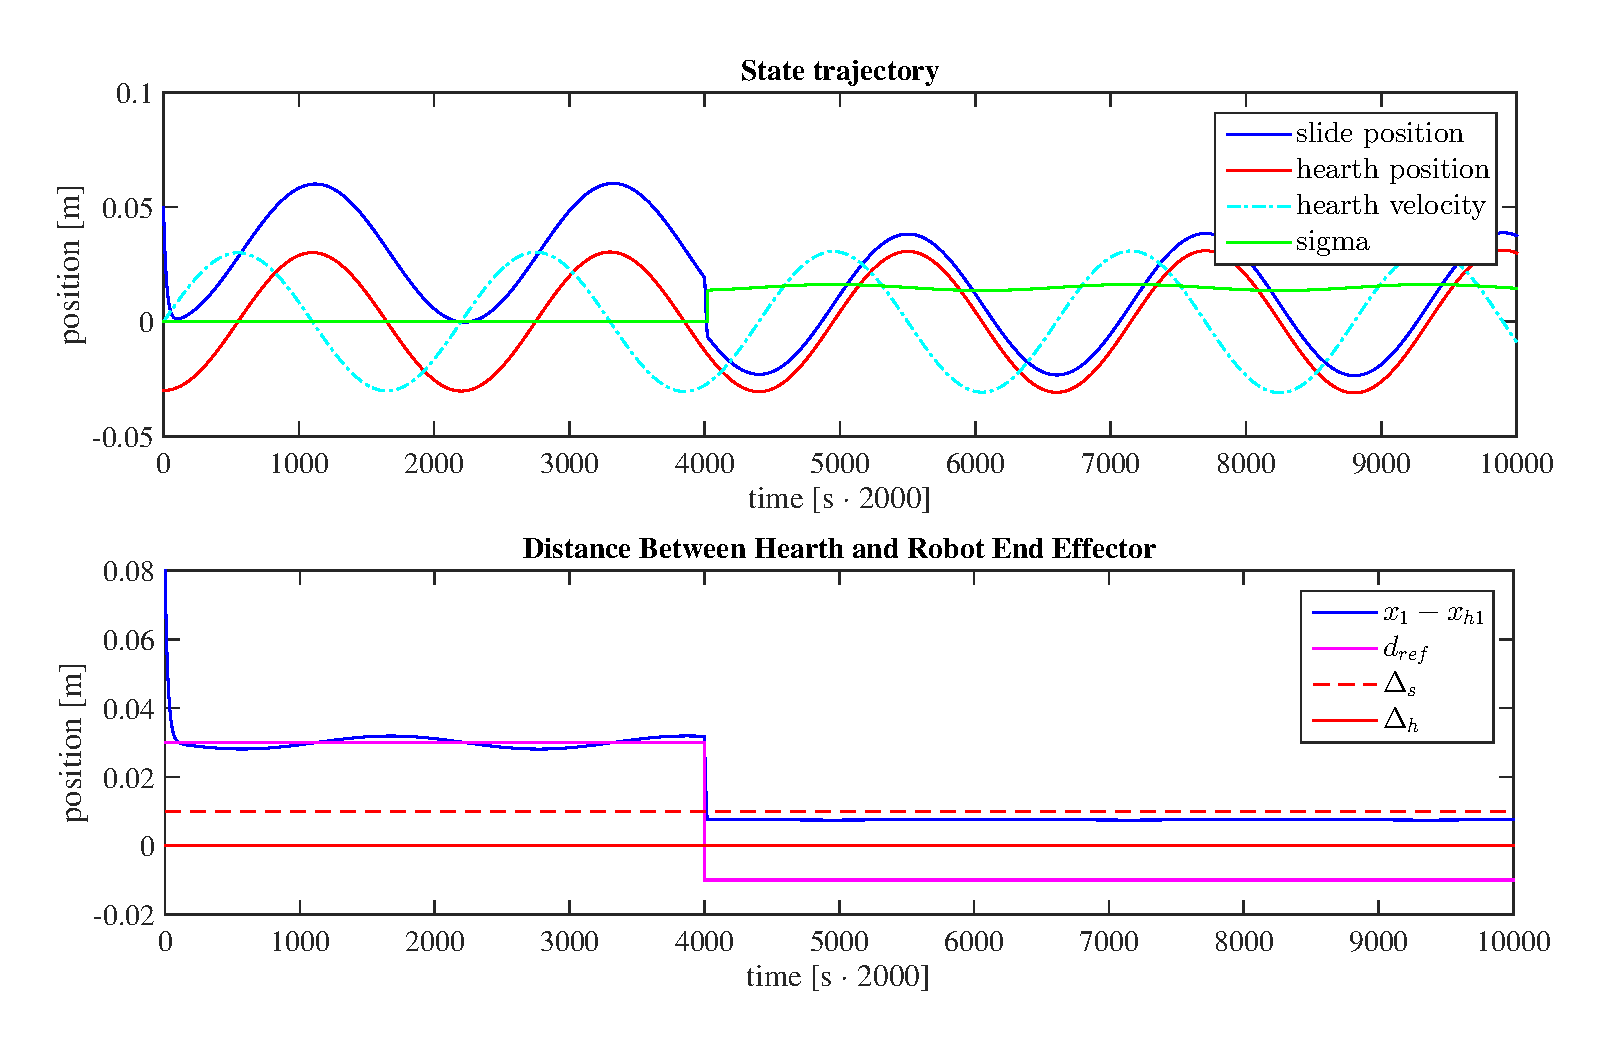
\includegraphics[width=1\textwidth]{state_trajectory_dynamic_matlab.eps}
	\caption{Dynamic system with heart position defined as the zero level set of the CBF. References are given as relative distances to the moving surface. When a reference outide the sage region is given, the safety controller prevents the tool from entering the unsafe region.}
    \label{fig:matlab_dynamics}
\end{figure}
It is from \autoref{fig:matlab_dynamics} seen that the robot end effector settles at a distance at $d_\text{ref}=3\,$cm until the simulation reaches 2\,s ($k=4000$). Then $d_\text{ref}$ changes to -1\,cm which causes the safety controller to react. The state $x_1$ settles at a safe distance from the beating heart which is left untouched, and the simulated controller is thereby verified to work as intended.

\section{Implementation on the Da Vinci Robot}

%\newpage
%%\begin{flalign}
%%f_{cl}(x)=\dot{\begin{bmatrix}
%%	x_1\\x_{h1}\\x_{h2}\\d_\text{ref}
%%	\end{bmatrix}} =
%%\underbrace{\underbrace{\begin{bmatrix}
%%		-1/\tau & 0 & 0 & 0\\0 & 0 & \omega_h & 0 \\ 0 & -\omega_h & 0 & 0 \\ 0& 0 & 0 & 0
%%		\end{bmatrix}}_{A}
%%	\begin{bmatrix}
%%	x_1\\x_{h1}\\x_{h2}\\d_\text{ref}
%%	\end{bmatrix}}_{f(x)}+ 
%%\underbrace{\underbrace{\begin{bmatrix}
%%		1/\tau \\ 0 \\ 0 \\ 0
%%		\end{bmatrix}}_{B}}_{g(x)}
%%\underbrace{\underbrace{\begin{bmatrix}
%%		-k & \bar{N} & 0 & \bar{N}
%%		\end{bmatrix}}_{K}
%%	\begin{bmatrix}
%%	x_1\\x_{h1}\\x_{h2}\\d_\text{ref}
%%	\end{bmatrix}}_{\tilde{u}(x)}
%%\end{flalign}
%%or formulated equivalently as
%%\begin{flalign}
%%\dot{\begin{bmatrix}
%%	x_1\\x_{h1}\\x_{h2}
%%	\end{bmatrix}} =
%%\underbrace{\begin{bmatrix}
%%	-(1+k)/\tau & \bar{N}/\tau & 0\\0 & 0 & \omega_h \\ 0 & -\omega_h & 0
%%	\end{bmatrix}}_{A_{cl}}
%%\begin{bmatrix}
%%x_1\\x_{h1}\\x_{h2}
%%\end{bmatrix}+ 
%%\underbrace{\begin{bmatrix}
%%	\bar{N}/\tau \\ 0 \\ 0
%%	\end{bmatrix}}_{B_{cl}}
%%d_{ref}
%%\end{flalign}
%%\begin{tabular}{rl}
%%where &\\
%%$\tau$ & is the time constant of the first order system $\tau=0.11$\,s as given in \autoref{sec:model_slide}\\
%%$k$ & is the linear system controller designed according to \autoref{eq:K_1}\\
%%$\bar{N}$ & is the system gain found according to \autoref{eq:barm_1}
%%\end{tabular}\\
%
%
%
%%
%%where $x_{h1}$ is the position of a point on the surface of the heart and $x_{h2}$ is the velocity of the point.
%%Here $\omega_h$ represents the frequency of the heart, 
%%$\omega_h$ has an average heartbeat period of 1.1\,s \citep{bib:heart_berkeley}, 
%%$\omega_h$ is set to be $2\pi/1.1$. 
%%In \autoref{fig:1stordersys_dynamiclimits} the moving surface of the heart is plotted over time, offset to an axis of oscillation in -6\,cm relative to the slide position. This curve marks the boundary to the unsafe region below it, and crossing this curve (from the safe region above it) corresponds to penetrating the heart surface with the surgical instrument tip. Note that the flexibility of the surface of the heart, at contact with the rigid tool, is not considered in the scope of this thesis. 
%%
%%\begin{figure}[htbp]
%%	\centering
%%	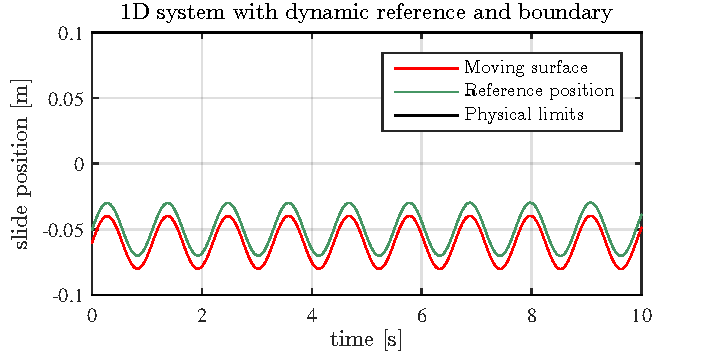
\includegraphics[width=0.65\textwidth]{1stordersys_dynamiclimits.pdf}
%%	\caption{Example of a moving surface representing the heart, marking the boundary to the unsafe region $\mathcal{X}_u$. A reference is set within the safe region as a fixed distance to the surface of the beating heart.}
%%	\label{fig:1stordersys_dynamiclimits}
%%\end{figure}
%%
%%In \autoref{fig:1stordersys_dynamiclimits} a sine amplitude of 2\,cm is used and the time dependent reference for the robot tool tip is defined as the heart position plus a fixed distance of 1\,cm in the positive slide direction $x_\text{ref}=x_{h1}+d_\text{ref}$, i.e. according to \autoref{eq:utilde} the linear position controller to be used in $\mathcal{X}_0$ is
%%\begin{equation}
%%\tilde{u}(t) = \bar{N}(x_{h1}(t)+d_\text{ref})-Kx(t) \label{eq:utilde_dynamic}
%%\end{equation}
%%\textcolor{red}{Or should it be $-k_1x_1$ no matter the order of the system?}
%%The reference distance can be picked as any nonnegative value still allowing the slide position to stay within its (upper) physical limit.
%The dynamic surface representing the heart also put forth new requirements to the safety controller, as the boundary between the safe and unsafe regions $\mathcal{X}_0$ and $\mathcal{X}_u$ (and thereby also the transition region $\mathcal{T}$ between the use of linear and safety controller) is now moving concurrently with the heart surface. This requires the construction of barrier certificates that are functions of robot state as well as the dynamic surface position.
%
%
%
%\section{Safe Controller Design for First Order System}
%First a linear position controller is designed for the augmented system consisting of the first order system modelled in \autoref{subsec:model_1d} and the simplified heart model in \autoref{eq:beating_heart_sine}. The controller is designed on the form presented in \autoref{eq:utilde}, and for the dynamic system, the reference is designed to be a fixed distance to the surface of the heart, as described in \autoref{eq:utilde_dynamic}.
%
%Once the closed-loop system has been designed, a barrier certificate is constructed iteratively by formulating a function that has its (dynamic) zero level set coinciding with the surface position of the heart, and is positive (indicating the unsafe region $\mathcal{X}_u$) below the surface and negative above, thus conforming with the first two requirements for a barrier certificate as given by \autoref{def:barrier_certificate}.
%
%In order to test compliance with the third requirement for a barrier certificate, the candidate barrier function is tested with the designed linear first order system according to the requirement in \autoref{req2}, and the candidate barrier function is altered iteratively until this requirement is fulfilled.
%
%When a barrier certificate for the closed-loop system has been found, a safety controller is designed according to \autoref{eq:control_law_safety}, and the region $\mathcal{T}$ is defined by choosing the constant $\epsilon$ and using the bump function $\sigma(x)$ in \autoref{eq:smoothness}, arriving at the safe controller in \autoref{eq:control_law} employing the linear position controller on $\mathcal{X}_0\setminus\mathcal{T}$ and the linear combination of the position controller and the CBF on $\mathcal{T}$
%
%\subsection{Setting up the Closed-Loop System and Designing the Linear Controller}
%An augmented state-space model including the dynamics of the robot tool from \autoref{eq:1storder_1D_ss} as well as the beating heart from \autoref{eq:beating_heart_sine}, is set up for the closed-loop first order system
%\begin{equation}
%f_{cl}(x)=\dot{\begin{bmatrix}
%	x_1\\x_{h1}\\x_{h2}\\d_\text{ref}
%	\end{bmatrix}} =
%\underbrace{\underbrace{\begin{bmatrix}
%		-1/\tau & 0 & 0 & 0\\0 & 0 & \omega_h & 0 \\ 0 & -\omega_h & 0 & 0 \\ 0& 0 & 0 & 0
%		\end{bmatrix}}_{A}
%	\begin{bmatrix}
%	x_1\\x_{h1}\\x_{h2}\\d_\text{ref}
%	\end{bmatrix}}_{f(x)}+ 
%\underbrace{\underbrace{\begin{bmatrix}
%		1/\tau \\ 0 \\ 0 \\ 0
%		\end{bmatrix}}_{B}}_{g(x)}
%\underbrace{\underbrace{\begin{bmatrix}
%		-k & \bar{N} & 0 & \bar{N}
%		\end{bmatrix}}_{K}
%	\begin{bmatrix}
%	x_1\\x_{h1}\\x_{h2}\\d_\text{ref}
%	\end{bmatrix}}_{\tilde{u}(x)}
%\end{equation}
%or formulated equivalently as
%\begin{equation}
%\dot{\begin{bmatrix}
%	x_1\\x_{h1}\\x_{h2}
%	\end{bmatrix}} =
%\underbrace{\begin{bmatrix}
%	-(1+k)/\tau & \bar{N}/\tau & 0\\0 & 0 & \omega_h \\ 0 & -\omega_h & 0
%	\end{bmatrix}}_{A_{cl}}
%\begin{bmatrix}
%x_1\\x_{h1}\\x_{h2}
%\end{bmatrix}+ 
%\underbrace{\begin{bmatrix}
%	\bar{N}/\tau \\ 0 \\ 0
%	\end{bmatrix}}_{B_{cl}}
%d_{ref}
%\end{equation}
%\begin{tabular}{rl}
%where &\\
%$\tau$ & is the time constant of the first order system $\tau=0.11$\,s as given in \autoref{sec:model_slide}\\
%$k$ & is the linear system controller designed according to \autoref{eq:K_1}\\
%$\bar{N}$ & is the system gain found according to \autoref{eq:barm_1}
%\end{tabular}\\
%
%\textcolor{red}{Should we design a $k$ that is slower conforming with what is found to be implementable?}
%
%Before designing the controller $k$, the stability of this system is analysed. \textcolor{red}{Be sure it's the same for reference as for estimated state!} In order for the system to be (asymptotically) stable, the error should converge to zero
%\begin{equation}
%e(t)=x_\text{ref}(t)-x_1(t)=x_{h1}(t)+d_\text{ref}-x_1(t) = 0 \label{eq:ref_error}
%\end{equation}
%The requirement of the system being stable can be tested as the derivative of the error converging to zero
%\vspace{-5mm}
%\begin{subequations}
%\begin{align}
%\dot{e}(t)=\dot{x}_\text{ref}(t)-\dot{x}_1(t)=\dot{x}_{h1}(t)-\dot{x}_1(t)
%&= \omega_h x_{h2}(t) - (-\tfrac{1}{\tau}x_1(t)+\tfrac{1}{\tau}\bar{N}x_\text{ref}(t-\tfrac{1}{\tau}kx_1(t)) \nonumber\\
%&= \omega_h x_{h2}(t) + \tfrac{1}{\tau}(1+k)x_1(t)-\tfrac{1}{\tau}\bar{N}x_\text{ref}(t)
%\end{align}
%For a first order system of this particular configuration of the $A$ and $B$ matrices, as seen from \autoref{eq:barm_1}, $\bar{N}=1+k$, reducing the equation to
%\begin{equation}
%\dot{e}(t) =\omega_h x_{h2}(t) + \tfrac{1}{\tau}\bar{N}(x_1(t)-x_\text{ref}(t) = \omega_h x_{h2}(t) - \tfrac{1}{\tau}\bar{N}e(t)
%\end{equation}
%Now setting the error derivative equal to zero
%\begin{align}
%0 &= \omega_h x_{h2}(t) - \tfrac{1}{\tau}\bar{N}e(t)\nonumber\\
%\tfrac{1}{\tau}\bar{N}e(t) &= \omega_h x_{h2}(t)\nonumber\\
%e(t) &= \frac{\omega_h \tau}{\bar{N}}x_{h2}(t)
%\end{align}
%The value of $x_{h2}$ is time dependent, but will have its maximum and minimum values in the amplitude of the sine, i.e. for a heart sine amplitude of $A_\text{heart}=2$\,cm $x_{h2}\in[-0.02,0.02]$\,m.
%\end{subequations}
%This means that the error will fluctuate between the values
%\begin{equation}
%e(t) \in \begin{bmatrix} -\frac{\omega_h \tau}{\bar{N}}A_\text{heart},  & \frac{\omega_h \tau}{\bar{N}}A_\text{heart}  \end{bmatrix}
%\end{equation}
%\textcolor{red}{Makes no sense! How can the error derivative be zero only when the error is fluctuating?!}
%From safety, $x_1$ should always be above $x_{h1}$, i.e.
%\begin{equation}
%x_1(t)\geq x_{h1}(t) \qquad \Leftrightarrow \qquad x_{h1}(t)-x_1(t)\leq 0
%\end{equation}
%and as seen from \autoref{eq:ref_error}, this puts up a safety requirement for the reference distance
%\begin{equation}
%x_{h1}(t)-x_1(t) = e(t)-d_\text{ref}\leq 0 \qquad \Leftrightarrow \qquad d_\text{ref}\geq e_\text{max}=\frac{\omega_h \tau}{\bar{N}}A_\text{heart}
%\end{equation}
%
%Stability analysis: test that the system has negative poles, i.e. that all $\lambda$s are negative for which
%\begin{equation}
%\det\begin{vmatrix}
%A_{cl}-\lambda I & B_{cl}\\C_{cl}&D_{cl}
%\end{vmatrix}=0
%\end{equation}
%As the output should be the robot tool position, i.e. $C_{cl}=[1\,\,\,0\,\,\,0]$ and $D_{cl}=0$, this is found as
%\begin{align}
%&\det\begin{vmatrix}
%-(1+k)/\tau-\lambda & \bar{N}/\tau & 0 & \bar{N}/\tau\\
%0 & -\lambda  & \omega_h  & 0\\ 
%0 & -\omega_h & -\lambda & 0\\
%1 & 0 & 0 & 0
%\end{vmatrix}
%= 
%%(-(1+k)/\tau-\lambda) \cdot
%%\begin{vmatrix}
%%-\lambda  & \omega_h  & 0\\ 
%%-\omega_h & -\lambda & 0\\
%%0 & 0 & 0
%%\end{vmatrix}
%-1 \cdot \det\begin{vmatrix}
%\bar{N}/\tau & 0 & \bar{N}/\tau\\
%-\lambda & \omega_h  & 0\\ 
%-\omega_h & -\lambda & 0\\
%\end{vmatrix} \nonumber\\
%&\phantom{det}= -1\cdot \frac{\bar{N}}{\tau} \cdot \det 
%\begin{vmatrix}
%-\lambda & \omega_h\\
%-\omega_h &  -\lambda\\
%\end{vmatrix}
%= -\frac{\bar{N}}{\tau} \cdot (\lambda^2 +\omega_h^2)
%= 0 \qquad \Leftrightarrow \qquad \lambda = \pm\omega_h
%\end{align}
%\textcolor{red}{Not stable! positive eigenvalue in $\omega_h$}
%
%\subsection{Constructing a Control Barrier Function}
%As mentioned, a barrier certificate for this system with a zero level set at the surface of the heart, comprises moving boundaries and hence should be a function of both robot and heart position. According to \autoref{def:safety} a $B(x_1,x_{h1})$ should be constructed with unsafe region $\mathcal{X}_u$ below the surface of the heart, i.e. such that $B(x_1,x_{h1})$ is positive if $x_1<x_{h1}$ and negative otherwise. The very simplest function satisfying this requirement is a function
%\begin{equation}
%B_0(x_1,x_{h1})= c(x_{h1}-x_1)
%\end{equation}
%with a positive constant $c>0$. This would result in the Lie derivatives % $L_{f_{cl}}B_0(x)$
%\begin{subequations}
%\begin{align}
%L_fB_0(x) &= \frac{dB_0(x)}{dx}f(x) =
%\begin{bmatrix}
%-c & c & 0 & 0
%\end{bmatrix}
%\begin{bmatrix}
%-x_1/\tau\\
%\omega_h x_{h2} \\
%-\omega_h x_{h1} \\
%0
%\end{bmatrix}=
%c\left(\omega_h x_{h2} + \frac{ x_1}{\tau}\right)\\
%L_gB_0(x) &= \frac{dB(x)}{dx}g(x) =
%\begin{bmatrix}
%-c & c & 0 & 0
%\end{bmatrix}
%\begin{bmatrix}
%1/\tau\\
%0 \\ 0 \\ 0
%\end{bmatrix}=
%\frac{-c}{\tau}\\
%L_{f_{cl}}B_0(x) & 
%%=\frac{dB_0(x)}{dx}f_{cl}(x) 
%= L_fB_0(x)+L_gB_0(x)u = 
%%\begin{bmatrix}
%%	-c & c & 0 & 0
%%\end{bmatrix}
%%\begin{bmatrix}
%%\frac{\bar{N}(x_{h1}+d_{ref})-(1+k) x_1}{\tau} \\
%%\omega_h x_{h2} \\
%%-\omega_h x_{h1}
%%\end{bmatrix}=
%c\left(\omega_h x_{h2} - \frac{\bar{N}(x_{h1} + d_{ref})-(1+k) x_1}{\tau}\right)
%\end{align}
%\end{subequations}
%The Lie derivative $L_{f_{cl}}B_0(x)$ (with the heart sine placed as in \autoref{fig:1stordersys_dynamiclimits}) should be negative for  $x_1\in[-0.1,0.1]$, $x_{h1}\in [-0.08,-0.04]$ and $x_{h2}\in [-0.02,0.02]$. We thus require that (recall from \autoref{eq:barm_1} that $\bar{N}=K+1$ for the present first order system)
%\begin{align}
%\omega_h x_{h2} &< \frac{\bar{N}(x_{h1} + d_{ref})-(1+k) x_1}{\tau} = \frac{1+k}{\tau}(x_{h1} + d_{ref}-x_1)\nonumber\\
%\omega_h x_{h2} \frac{\tau}{1+k} &< x_{h1} + d_{ref}-x_1
%\end{align}
%With the largest positive value of $x_{h2}=0.02$\,m and the same controller $K=9$ is used as in \autoref{eq:K_1}, the left-hand expression attains a largest value of 0.00126\,m, requiring that the error between the robot tool position and the reference position always be slightly larger than a millimeter. 
%%2*pi/1.1*0.02/(10/0.11)
%%0.001256637061436
%Obviously this barrier function is not valid, and a different function is opted for.
%
%According to \cite{bib:org_control} a barrier certificate might be found iteratively by using $B_0(x)$ in the construction of a barrier certificate on the form
%\begin{equation}
%B(x) = 
%\begin{cases}
%B_0(x) & \text{if}\quad L_fB_0(x) \leq -\beta\\
%B_0(x)+\alpha(L_fB_0(x)+\beta)^2 & \text{if}\quad L_fB_0(x)>-\beta 
%\end{cases}
%\end{equation}
%where $\alpha>0$, $\beta>0$ are parameters to be determined. For the presented system this gives the barrier candidate function 
%\begin{equation}
%B(x) = 
%\begin{cases}
%c(x_{h1}-x_1) & \text{if}\quad c\left(\omega_h x_{h2} +  x_1/\tau\right) \leq -\beta\\
%c(x_{h1}-x_1)+\alpha(c\left(\omega_h x_{h2} +  x_1/\tau\right)+\beta)^2 & \text{if}\quad c\left(\omega_h x_{h2} +  x_1/\tau\right)>-\beta 
%\end{cases}
%\end{equation}
%\textcolor{red}{The constant $c$ is unimportant. Set $c=1$.  In the example in \citep{bib:org_control} they chose $\alpha=1/20$ and $\beta=1$, giving}
%\begin{equation}
%B(x) = 
%\begin{cases}
%x_{h1}-x_1 & \text{if}\quad x_1 \leq -0.11-0.2\pi x_{h2}\\
%x_{h1}-x_1+\dfrac{1}{20}\left(\dfrac{0.2\pi\,\, x_{h2} +   x_1}{0.11}+1\right)^2 & \text{if}\quad x_1 > -0.11-0.2\pi x_{h2} 
%\end{cases}
%\end{equation}
%\textcolor{red}{Need to test this!}
%
%
%\section{Safe Controller Design for Second Order System}
%\textcolor{red}{introduce}
%
%\subsection{Setting up the Closed-Loop System and Designing the Linear Controller}
%As for the first order system, the second order system in \autoref{eq:2ndorder_1D_ss} is augmented with the dynamics of the beating heart and with the reference given as a fixed distance from the surface of the beating heart
%\begin{equation}
%\dot{\begin{bmatrix}
%x_1\\x_2\\x_{h1}\\x_{h2}
%\end{bmatrix}} = \begin{bmatrix}
%0 & 1 & 0 & 0\\
%-\omega_n^2(1+k_1)  & -2\zeta \omega_n-\omega_n^2 k_2  & \omega_n^2\bar{N} & 0\\
%0 & 0 & 0 & \omega_h \\
%0 & 0 & -\omega_h & 0
%\end{bmatrix}\begin{bmatrix}
%x_1\\x_2\\x_{h1}\\x_{h2}
%\end{bmatrix} + \begin{bmatrix}
%0\\\omega_n^2\bar{N} \\ 0 \\ 0
%\end{bmatrix}d_{ref}
%\end{equation}
%\begin{tabular}{rl}
%where &\\
%$\omega_n$ & is the natural frequency of the second order system $\omega_n=17$\,rad/s as given in \autoref{sec:model_slide}\\
%$\zeta$ & is the damping ratio of the second order system $\zeta=0.05$ as given in \autoref{sec:model_slide}\\
%$[k_1\,\,\,k_2]$ & is the linear system controller designed according to \autoref{eq:K_2}\\
%$\bar{N}$ & is the system gain found according to \autoref{eq:Nbar_2}
%\end{tabular}\\
%
%
%Can also be written on augmented form where the reference is part of the state
%\begin{equation}
%\dot{\begin{bmatrix}
%	x_1\\x_2\\x_{h1}\\x_{h2}\\d_{ref}
%	\end{bmatrix}} = 
%\underbrace{\underbrace{\begin{bmatrix}
%		0 & 1 & 0 & 0 & 0\\
%		-\omega_n^2  & -2\zeta \omega_n  & 0 & 0 & 0\\
%		0 & 0 & 0 & \omega_h & 0\\
%		0 & 0 & -\omega_h & 0 & 0\\
%		0 & 0 & 0 & 0 & 0
%		\end{bmatrix}}_{A}
%	\begin{bmatrix}
%	x_1\\x_2\\x_{h1}\\x_{h2}\\d_{ref}
%	\end{bmatrix}}_{f(x)} + 
%\underbrace{\underbrace{\begin{bmatrix}
%		0\\\omega_n^2 \\ 0 \\ 0 \\ 0
%		\end{bmatrix}}_{B}}_{g(x)}
%\underbrace{\underbrace{\begin{bmatrix}
%		-k_1 & -k_2 & \bar{N} & 0 & \bar{N}
%		\end{bmatrix}}_{K}
%	\begin{bmatrix}
%	x_1\\x_2\\x_{h1}\\x_{h2}\\d_{ref}
%	\end{bmatrix}}_{u}
%\end{equation}